%%%%%%%%%%%%%%%%%%%%%%%%%%%%%%%%%%%%%%%%%%%%%%%%%%%%%%%%%%%%%%%%%%%%%%%%%%%%
% AGUJournalTemplate.tex: this template file is for articles formatted with LaTeX
%
% This file includes commands and instructions
% given in the order necessary to produce a final output that will
% satisfy AGU requirements, including customized APA reference formatting.
%
% You may copy this file and give it your
% article name, and enter your text.
%
%
% Step 1: Set the \documentclass
%
%

%% To submit your paper:
\documentclass[draft]{agujournal2019}
\usepackage{url} %this package should fix any errors with URLs in refs.
\usepackage{lineno}
\usepackage[inline]{trackchanges} %for better track changes. finalnew option will compile document with changes incorporated.
\usepackage{soul}
\linenumbers
%%%%%%%
% As of 2018 we recommend use of the TrackChanges package to mark revisions.
% The trackchanges package adds five new LaTeX commands:
%
%  \note[editor]{The note}
%  \annote[editor]{Text to annotate}{The note}
%  \add[editor]{Text to add}
%  \remove[editor]{Text to remove}
%  \change[editor]{Text to remove}{Text to add}
%
% complete documentation is here: http://trackchanges.sourceforge.net/
%%%%%%%

\draftfalse

%% Enter journal name below.
%% Choose from this list of Journals:
%
% JGR: Atmospheres
% JGR: Biogeosciences
% JGR: Earth Surface
% JGR: Oceans
% JGR: Planets
% JGR: Solid Earth
% JGR: Space Physics
% Global Biogeochemical Cycles
% Geophysical Research Letters
% Paleoceanography and Paleoclimatology
% Radio Science
% Reviews of Geophysics
% Tectonics
% Space Weather
% Water Resources Research
% Geochemistry, Geophysics, Geosystems
% Journal of Advances in Modeling Earth Systems (JAMES)
% Earth's Future
% Earth and Space Science
% Geohealth
%
% ie, \journalname{Water Resources Research}

\journalname{Enter journal name here}

%%%%% PERSONNAL MACROS and ENVIRONMENTS %%%%%%

\usepackage{bm} %bold symbols and letters in math mode, that stays italicized
%\usepackage{dutchcal} % \mathcal: also small letters. \mathbcal = bold ones. 
\DeclareFontFamily{OT1}{pzc}{}
\DeclareFontShape{OT1}{pzc}{m}{it}{<-> s * [1.10] pzcmi7t}{}
\DeclareMathAlphabet{\mathpzc}{OT1}{pzc}{m}{it}

\usepackage{amsmath}
\usepackage{colortbl}

\usepackage{subfiles}
\usepackage{graphicx}
\graphicspath{{images/}} %for subfile graphics

\usepackage{siunitx} %SI units !
\sisetup{detect-all}
% \usepackage{biblatex}

\usepackage{caption}
%\usepackage{subcaption} %for subfigures 

%Delimiters
\newcommand\restrict[1]{\raisebox{-.5ex}{$|$}_{#1}} %restriction to a value 
\newcommand{\an}[1]{\ensuremath{\left\langle#1\right\rangle}} %angles
\newcommand{\sbra}[1]{\ensuremath{\left[#1\right]}} %square brackets []
\newcommand{\pbra}[1]{\ensuremath{\left\{#1\right\}}} %Poisson bracket {}
\newcommand{\parenthese}[1]{\ensuremath{\left(#1\right)}} %parentheses
\newcommand{\abs}[1]{\ensuremath{\left |#1\right |}} %absolute value

%Math Symbols
\newcommand{\g}{\mathbf{g}}
\newcommand{\dd}{\mathrm{d}}
\newcommand{\uu}{\tilde{u}}
\newcommand{\ww}{\tilde{w}}
\newcommand{\pp}{\tilde{p}}
\newcommand{\Ak}{\hat{A}_k}
\newcommand{\HH}{\mathcal{H}}
\newcommand{\ee}{{\rm e}}
\newcommand{\ii}{{\rm i}}
\newcommand{\Ks}{K_{\overline{\Sigma}}}
\newcommand{\R}{\mathbb{R}}
\newcommand{\ga}{\mathbf{\gamma}}
\newcommand{\al}{\mathbf{\alpha}}
\newcommand{\bb}{\mathbf{\beta}}
\newcommand{\K}{\mathbb{K}}


%Colored text
\definecolor{BlueGreen}{cmyk}{0.85,0,0.33,0}
\newcommand{\blu}[1]{{\color{BlueGreen} #1}}
\newcommand{\rose}[1]{{\color{magenta} #1}}    
\definecolor{mycolor}{RGB}{252,186,3}
\newcommand{\oran}[1]{{\color{mycolor} #1}}

%\usepackage{refcheck}
%%%
\definecolor{DodgerBlue}{RGB}{30,144,255}
\definecolor{peru}{RGB}{205,133,63}
%%%
\newcommand{\FLcom}[1]{\textcolor{DodgerBlue}{~\textit{(\textbf{FL:}~{#1})}}}
\newcommand{\FLadd}[1]{\textcolor{peru}{{#1}}}              
\newcommand{\FLdel}[1]{\textcolor{peru}{\sout{{#1}}}}     

%%%%%%%%%%%%%%%%%%%%%%%%%%%%%%%%%%%%%%%%%%%%%%%%%%%%%%%%%%%%%%
%%%%%%%%%%%%%%%%%%%%%%%%%%%%%%%%%%%%%%%%%%%%%%%%%%%%%%%%%%%%%%




\begin{document}

%% ------------------------------------------------------------------------ %%
%  Title
%
% (A title should be specific, informative, and brief. Use
% abbreviations only if they are defined in the abstract. Titles that
% start with general keywords then specific terms are optimized in
% searches)
%
%% ------------------------------------------------------------------------ %%

% Example: \title{This is a test title}

\title{Prior constraints and Bayesian estimation for an oceanic parameterization}

%% ------------------------------------------------------------------------ %%
%
%  AUTHORS AND AFFILIATIONS
%
%% ------------------------------------------------------------------------ %%

% Authors are individuals who have significantly contributed to the
% research and preparation of the article. Group authors are allowed, if
% each author in the group is separately identified in an appendix.)

% List authors by first name or initial followed by last name and
% separated by commas. Use \affil{} to number affiliations, and
% \thanks{} for author notes.
% Additional author notes should be indicated with \thanks{} (for
% example, for current addresses).

% Example: \authors{A. B. Author\affil{1}\thanks{Current address, Antartica}, B. C. Author\affil{2,3}, and D. E.
% Author\affil{3,4}\thanks{Also funded by Monsanto.}}

\authors{=list all authors here=}


% \affiliation{1}{First Affiliation}
% \affiliation{2}{Second Affiliation}
% \affiliation{3}{Third Affiliation}
% \affiliation{4}{Fourth Affiliation}

\affiliation{=number=}{=Affiliation Address=}
%(repeat as many times as is necessary)

%% Corresponding Author:
% Corresponding author mailing address and e-mail address:

% (include name and email addresses of the corresponding author.  More
% than one corresponding author is allowed in this LaTeX file and for
% publication; but only one corresponding author is allowed in our
% editorial system.)

% Example: \correspondingauthor{First and Last Name}{email@address.edu}

\correspondingauthor{=name=}{=email address=}

%% Keypoints, final entry on title page.

%  List up to three key points (at least one is required)
%  Key Points summarize the main points and conclusions of the article
%  Each must be 140 characters or fewer with no special characters or punctuation and must be complete sentences

% Example:
% \begin{keypoints}
% \item	List up to three key points (at least one is required)
% \item	Key Points summarize the main points and conclusions of the article
% \item	Each must be 140 characters or fewer with no special characters or punctuation and must be complete sentences
% \end{keypoints}

\begin{keypoints}
\item enter point 1 here
\item enter point 2 here
\item enter point 3 here
\end{keypoints}

%% ------------------------------------------------------------------------ %%
%
%  ABSTRACT and PLAIN LANGUAGE SUMMARY
%
% A good Abstract will begin with a short description of the problem
% being addressed, briefly describe the new data or analyses, then
% briefly states the main conclusion(s) and how they are supported and
% uncertainties.

% The Plain Language Summary should be written for a broad audience,
% including journalists and the science-interested public, that will not have 
% a background in your field.
%
% A Plain Language Summary is required in GRL, JGR: Planets, JGR: Biogeosciences,
% JGR: Oceans, G-Cubed, Reviews of Geophysics, and JAMES.
% see http://sharingscience.agu.org/creating-plain-language-summary/)
%
%% ------------------------------------------------------------------------ %%

%% \begin{abstract} starts the second page

\begin{abstract}
[ enter your Abstract here ]
\end{abstract}

\section*{Plain Language Summary}
[ enter your Plain Language Summary here or delete this section]


%% ------------------------------------------------------------------------ %%
%
%  TEXT
%
%% ------------------------------------------------------------------------ %%


\section{Introduction}

\section{Description of the parameterization}

In this section, we briefly expose the single-column model (SCM) and the parameterization of its turbulence via the EDMF approach proposed in \citeA{perrotEnergeticallyConsistentEddyDiffusivity2024}. The evolution equations for mean conservative temperature $\overline{\theta}$, salt $\overline{S}$ and horizontal velocities $\overline{\bm u}_h = (\overline{u},\overline{v})$ are 
%
\begin{eqnarray*}
    \begin{cases}
        \partial_t \overline{\theta} = \frac{\overline{\epsilon}_\nu }{c_p - \alpha gz } - \partial_z \overline{w' \theta'} \label{eq:temp budget}
        \\
        \partial_t \overline{S} = - \partial_z \overline{w' S'}
        \\
        \partial_t \overline{\bm u}_h = - \partial_z \overline{w' \bm u_h'} - f \bm e_z \times \overline{\bm u}
    \end{cases}
\end{eqnarray*}
%
where $alpha$ and $c_p$ are respectively the thermal expansion coefficient and specific heat capacity of seawater. Although of negligible importance in the ocean, the non-classical viscous heating due to the dissipation of turbulence $\overline{\epsilon}$ is retained to achieve  properly closed energy budgets between mean and turbulent kinetic energy \cite{perrotEnergeticallyConsistentEddyDiffusivity2024}. The turbulent fluxes of the form $\overline{w'X'}$ (with $X=\theta,S,\bm u_h$) are closed according to the Eddy-Diffusivity Mass-Flux (EDMF) parameterization:
%
\begin{eqnarray*}
    \overline{w'X'} = \underbrace{-K_X \partial_z \overline{X}}_{\rm{ED}} + \underbrace{a_p w_p (X_p - \overline{X})}_{\rm{MF}}
\end{eqnarray*}
%
In the present study, the eddy viscosity $K_u$ and diffusivities $K_\theta=K_S$ 
in turbulent vertical fluxes are computed from a turbulence closure model based on a 
prognostic equation for the turbulent kinetic energy (TKE) 
$\displaystyle k = \overline{{\bm u}' \cdot {\bm u}'} / 2$ and a diagnostic 
computation of appropriate length scales (a.k.a. 1.5-order turbulence closure; see \citeA{perrotEnergeticallyConsistentEddyDiffusivity2024} for details). The plume fractional area, velocities, temperature and salinity $a_p, u_p, v_p,w_p, \theta_p, S_p$ are computed via the following system of ODEs
%
\begin{eqnarray*}
    \begin{cases}
        \partial_z (a_p w_p) = E-D
        \\
        a_p w_p \partial_z \theta_p = E (\overline{\theta} - \theta_p)
        \\
        a_p w_p \partial_z S_p = E (\overline{S} - S_p)   
        \\
        a_p w_p \partial_z \bm u_{h,p} = E (\overline{\bm u}_h - \bm u_{h,p}) + a_p w_p \underline{C_u} \partial_z   \overline{\bm u}_h 
        \\
        a_p w_p \partial_z w_p = - \underline{b} E w_p + \underline{a} a_p (b_{\rm{eos}}(\theta_p, S_p) - b_{\rm{eos}}(\overline{\theta},\overline{S}) ) +\underline{ b'} \frac{1}{h} a_p (w_p)^2 
        \\
        E = a_p \underline{C_{\epsilon}} \max (0,\partial_z w_p)
        \\
        D = -a_p \underline{C_{\delta}} \min (0,\partial_z w_p) - a_p w_p \underline{\delta_0}\frac{1}{h}
    \end{cases}
\end{eqnarray*}
%
where $h(t)$ is a plume vertical length, computed as the depth at which $w_p$ reaches a minimum value $w_p^{\rm min}$. \blu{TODO: use wp0 as a paramter, different from wpmin !!} The imposed surface plume fraction $a_p(z=0)=\underline{a_p^0}$ and plume vertical velocity $w_p(z=0) = \underline{w_p^0}$ provide two additional parameters. Consequently the parameters to estimate forms an array $\bm C = (C_\epsilon, C_\delta, C_u, a, b, b', \delta_0, a_p^0, w_p^0)$. Note that the TKE equation contains also adjustable parameters. However we do not include them in the estimation procedure, since we aim to recover the standard TKE scheme in non convective conditions.  


% Finally, the parameterized TKE equation is
% %
% \begin{eqnarray*}
%     \partial_t k + \partial_z  T_k =   - K_\phi \partial_z \overline{b} + a_p w_p (b_p - \overline{b}) + K_u (\partial_z \overline{\bm u}_h)^2 - a_p w_p (\bm u_{h,p} - \overline{\bm u}_h) \cdot \partial_z \overline{\bm u}_h - \overline{\epsilon}_{\nu}   
% \end{eqnarray*}
% %
% where the TKE flux is 
% %
% \begin{eqnarray*}
%     T_k &=& - K_k \partial_z k
%     + a_p w_p  \parenthese{k_p - k + \frac{1}{2} \| \bm u_p - \overline{\bm u} \|^2}  
% \end{eqnarray*}



\section{A priori constraints on parameters}
%
\subsection{$C_\epsilon$ and $C_\delta$}

\blu{Is the constraint exposed in appendix of the paper is related to the dicsretization, or is it possible to get the continuous analog?}

Constraints on $C_\epsilon$ and $C_\delta$ can be derived from the physical constraint $0\leq a_p \leq 1$. A sufficient condition to ensure that $a_p \leq 1$ at any depth is to impose $\partial_z a_p \geq 0$. It would imply that $a_p(z) \leq a_p(z=0)$ for any $z \leq 0$. Rewriting the $a_p$ equation as
%
\begin{eqnarray*}
    \partial_z a_p = a_p \delta_0 + 
    \begin{cases}
        (1-C_\epsilon) a_p \frac{\partial_z w_p}{-w_p} \text{ if } \partial_z w_p \geq 0
        \\
        (1-C_\delta) a_p \frac{\partial_z w_p}{-w_p} \text{ if } \partial_z w_p < 0             
    \end{cases}
\end{eqnarray*}
%
Recalling that $w_p<0$, sufficient conditions to have $\partial_z a_p \geq0$ are $C_\epsilon \leq 1$, $C_\delta \geq 1$ and $\delta_0 \geq 0$. Next we rewrite the $a_p$ equation as
%
\begin{eqnarray*}
    a_p = \partial_z a_p \parenthese{ \delta_0 +  
    \begin{cases}
        (1-C_\epsilon)\frac{\partial_z w_p}{-w_p} \text{ if } \partial_z w_p \geq 0
        \\
        (1-C_\delta)  \frac{\partial_z w_p}{-w_p} \text{ if } \partial_z w_p < 0              \end{cases}
    }
\end{eqnarray*}
%
We deduce that sufficient conditions to impose $a_p\geq 0$ when $\partial_z a_p \geq 0$ are once again $C_\epsilon \leq 1$, $C_\delta \geq 1$ and $\delta_0 \geq 0$. \blu{la condition $C_\delta < 2$ vient de la dicsrétisation avec $\Delta z E = 1/2 (a^p_+ + a^p_-) C_\epsilon (\delta_z w^p)^+$. C'est plus une contrainte numérique que physique...}. 

\subsection{$C_u$}
%
In this subsection, we provide global energy budgets to highlight the role of mass-flux terms in bulk energy 
exchange as well as sinks/sources at boundaries. Let us introduce the vertical average 
$\an{ X }_z = 1/H\int_{- H}^0 X  \, \dd z$, and the boundary operator
$\sbra{X}_{- H}^0 = 1/ H (X(z=0) - X(z=-H) )$. Then after some algebra we have
%
\begin{eqnarray*}
    \partial_t \an{ E_k }_z &=& - \an{  K_u (\partial_z \overline{\bm u}_h)^2  }_z - \an{ \frac{E + D}{2 (1-C_u) } (\bm u_{h,p} - \overline{\bm u}_h)^2 }_z 
\\
 &&  - \sbra{ \overline{\bm u}_h \cdot \overline{w'\bm u_h' } }_{- H}^0- \sbra{ \frac{a_p w_p}{2 (1- C_u)} (\bm u_{h,p} - \overline{\bm u}_h)^2  }_{- H}^0
\end{eqnarray*}
%
Since the term $- \an{ \frac{E + D}{2 (1-C_u) } (\bm u_{h,p} - \overline{\bm u}_h)^2 }_z $ is associated to a transfer from mean kinetic energy to TKE due to entrainent and detrainment processes, it should remain negative. Thus it implies that $C_u < 1$. Additionally, we must impose $C_u \geq 0$ \cite{wuEffectsVerticalWind1994}.  \blu{\cite{wuEffectsVerticalWind1994} indique en fait que $C_u$ et $C_v$ dépendent de la géométrie de l'écoulement. Typiquement pour des rouleaux selon $x$ $C_u < 2$ et $C_v=0$...}

\subsection{$a$ and $b$}

The parameters $a$ and $b$ have been introduced respectively as reduced a virtual mass term \cite<e.g.>{brethertonNewParameterizationShallow2004} – representing the reduction of plume
buoyancy due to pushing and pulling on the environment – and a reduced entrainment term. Thus by definition we have 
%
\begin{eqnarray*}
    0 \leq a < 1, \quad  0 \leq b < 1
\end{eqnarray*}

\subsection{$b'$ and $\delta_0$}

Compared to the original version exposed in \cite{perrotEnergeticallyConsistentEddyDiffusivity2024}, the terms involving $b'$ and $\delta_0$ has been rescaled by $\frac{1}{h}$ to obtain non-dimensional parameters.


\subsection{}




\section{Bayesian estimation method}
We estimate the optimal parameters using Bayesian inference method.
Instead of a single estimation point, this gives us a distribution of possible parameter values together with the likelihood of them being optimal.
We start with a prior distribution on the parameters, from the section above,
\begin{equation*}
	\pi_{\text{prior}}(\bm C).
\end{equation*}
Given our model, we introduce the Likelihood function
\begin{equation}
	\mathcal{L}(\bm y | \bm C)
\end{equation}

\section{Sobol' Indices}

Compute the variance/sensitivity of $Y=f(X)$ wrt to $X$. One can use the prior distribution. But one can also use the posterior distribution to sample $X$. Thus if $X_1$ has a small variance (meaning that we have learned from the data the distribution with good accuracy), posterior Sobol indices  assess if the model is sensitive or not to the remaining uncertainty (ie the variance) of the distribution of $X_1$. 
\\
\blu{This is NOT WORKING since inputs needs to be independent! }
Alternatives:
\begin{itemize}
    \item Shapley indices: Clementine's book provide implementation in R. But the problem is that it will work for point-wise scalar product, not L2 scalar product
    \item Global Sobol' indices ? 
\end{itemize}

To assess the quality of the estimation, we can also cross-validate with additional observations.

\section{Numerical results}
%
\begin{itemize}
    \item MAP
    \item showing the panel with posterior distribution
    \item uncertianty andrew plot (check souza)
    \item compute confidence intervals and trsholded prameters range on the marginal posterior
\end{itemize}
\section{Discussion}

\section{Conclusion}

%%% Suggested section heads:
% \section{Introduction}
%
% The main text should start with an introduction. Except for short
% manuscripts (such as comments and replies), the text should be divided
% into sections, each with its own heading.

% Headings should be sentence fragments and do not begin with a
% lowercase letter or number. Examples of good headings are:

% \section{Materials and Methods}
% Here is text on Materials and Methods.
%
% \subsection{A descriptive heading about methods}
% More about Methods.
%
% \section{Data} (Or section title might be a descriptive heading about data)
%
% \section{Results} (Or section title might be a descriptive heading about the
% results)
%
% \section{Conclusions}


\section{= enter section title =}
%Text here ===>>>


%%

%  Numbered lines in equations:
%  To add line numbers to lines in equations,
%  \begin{linenomath*}
%  \begin{equation}
%  \end{equation}
%  \end{linenomath*}



%% Enter Figures and Tables near as possible to where they are first mentioned:
%
% DO NOT USE \psfrag or \subfigure commands.
%
% Figure captions go below the figure.
% Table titles go above tables;  other caption information
%  should be placed in last line of the table, using
% \multicolumn2l{$^a$ This is a table note.}
%
%----------------
% EXAMPLE FIGURES
%
% \begin{figure}
% \includegraphics{example.png}
% \caption{caption}
% \end{figure}
%
% Giving latex a width will help it to scale the figure properly. A simple trick is to use \textwidth. Try this if large figures run off the side of the page.
% \begin{figure}
% \noindent\includegraphics[width=\textwidth]{anothersample.png}
%\caption{caption}
%\label{pngfiguresample}
%\end{figure}
%
%
% If you get an error about an unknown bounding box, try specifying the width and height of the figure with the natwidth and natheight options. This is common when trying to add a PDF figure without pdflatex.
% \begin{figure}
% \noindent\includegraphics[natwidth=800px,natheight=600px]{samplefigure.pdf}
%\caption{caption}
%\label{pdffiguresample}
%\end{figure}
%
%
% PDFLatex does not seem to be able to process EPS figures. You may want to try the epstopdf package.
%

%
% ---------------
% EXAMPLE TABLE
% Please do NOT include vertical lines in tables
% if the paper is accepted, Wiley will replace vertical lines with white space
% the CLS file modifies table padding and vertical lines may not display well
%


%% SIDEWAYS FIGURE and TABLE
% AGU prefers the use of {sidewaystable} over {landscapetable} as it causes fewer problems.
%
% \begin{sidewaysfigure}
% \includegraphics[width=20pc]{figsamp}
% \caption{caption here}
% \label{newfig}
% \end{sidewaysfigure}
%
%  \begin{sidewaystable}
%  \caption{Caption here}
% \label{tab:signif_gap_clos}
%  \begin{tabular}{ccc}
% one&two&three\\
% four&five&six
%  \end{tabular}
%  \end{sidewaystable}




\section{Open Research}
AGU requires an Availability Statement for the underlying data needed to understand, evaluate, and build upon the reported research at the time of peer review and publication.

Authors should include an Availability Statement for the software that has a significant impact on the research. Details and templates are in the Availability Statement section of the Data and Software for Authors Guidance: \url{https://www.agu.org/Publish-with-AGU/Publish/Author-Resources/Data-and-Software-for-Authors#availability}

It is important to cite individual datasets in this section and, and they must be included in your bibliography. Please use the type field in your bibtex file to specify the type of data cited. Some options include Dataset, Software, Collection, ComputationalNotebook. Ex: 
\\

%%%%%%%%%%%%%%%%%%%%%%%%%%%%%%%%%%%%%%%%%%%%%%%

\acknowledgments
This section is optional. Include any Acknowledgments here.
The acknowledgments should list:\\
All funding sources related to this work from all authors\\
Any real or perceived financial conflicts of interests for any author\\
Other affiliations for any author that may be perceived as having a conflict of interest with respect to the results of this paper.\\
It is also the appropriate place to thank colleagues and other contributors. AGU does not normally allow dedications.


%% ------------------------------------------------------------------------ %%
%% References and Citations

%%%%%%%%%%%%%%%%%%%%%%%%%%%%%%%%%%%%%%%%%%%%%%%
%
% \bibliography{<name of your .bib file>} don't specify the file extension
%
% don't specify bibliographystyle

% In the References section, cite the data/software described in the Availability Statement (this includes primary and processed data used for your research). For details on data/software citation as well as examples, see the Data & Software Citation section of the Data & Software for Authors guidance
% https://www.agu.org/Publish-with-AGU/Publish/Author-Resources/Data-and-Software-for-Authors#citation

%%%%%%%%%%%%%%%%%%%%%%%%%%%%%%%%%%%%%%%%%%%%%%%

\bibliography{references}



%Reference citation instructions and examples:
%
% Please use ONLY \cite and \citeA for reference citations.
% \cite for parenthetical references
% ...as shown in recent studies (Simpson et al., 2019)
% \citeA for in-text citations
% ...Simpson et al. (2019) have shown...
%
%
%...as shown by \citeA{jskilby}.
%...as shown by \citeA{lewin76}, \citeA{carson86}, \citeA{bartoldy02}, and \citeA{rinaldi03}.
%...has been shown \cite{jskilbye}.
%...has been shown \cite{lewin76,carson86,bartoldy02,rinaldi03}.
%... \cite <i.e.>[]{lewin76,carson86,bartoldy02,rinaldi03}.
%...has been shown by \cite <e.g.,>[and others]{lewin76}.
%
% apacite uses < > for prenotes and [ ] for postnotes
% DO NOT use other cite commands (e.g., \citet, \citep, \citeyear, \citealp, etc.).
% \nocite is okay to use to add references from your Supporting Information
%

\appendix

\section{Quality of MCMC}
There are multiple qualitative and quantitative methods to evaluate the quality of MCMC results.
First, visually, we compare the \emph{mixing of different chains}.
To do so, we plot the sample density of different chains and see if they agree for all parameters.
\begin{figure}
	\centering
	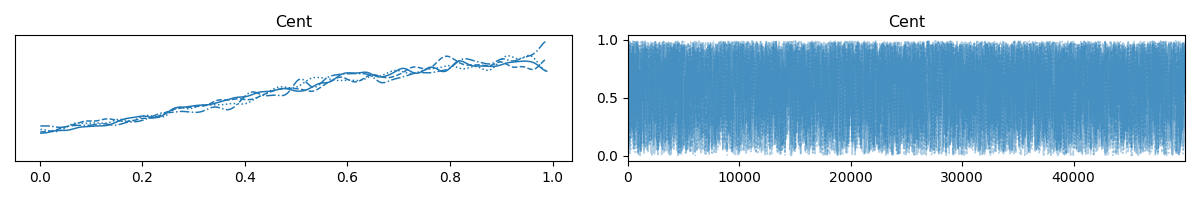
\includegraphics[width=\textwidth]{figures/Cent_trace.png}
	\caption{Mixing of $4$ different MCMC chains. The densities for the given parameter (see left) agrees for all chains.}\label{fig:mixing_of_MCMC_chains}
\end{figure}
For an example, see Figure~\ref{fig:mixing_of_MCMC_chains}.
If the densities of the different chains do not agree well, this is an indicator that MCMC has not yet converged and more samples are needed.

Next, we look at more quantitative methods.
A widely used one is $\hat{R}$, which compares the variance in a chain with the variance between all chains.
Let $W_k$ be the variance and $E_k$ the expectation in the $k$-th chain.
Define the average chain variance $W$ and the between chains variance $B$ as
\begin{align}
	W &= \frac{1}{m} \sum_{k=1}^{m} W_{k} \\
	B &= \frac{1}{m-1} \sum_{k=1}^{m} \left(E_k - \frac{1}{m} \sum_{k=1}^{m} E_k\right)
\end{align}
and define
\begin{equation}
	\hat{R} = \sqrt{\frac{n-1}{n} + \frac{B}{W}}.
\end{equation}
Note that for $n \rightarrow \infty$, $B \rightarrow 0$, while this is not the case for $W$. Hence, a converged MCMC chain has a value close to $1$.

Finally, let us talk about the \emph{effective sample size (ESS)}.
This quantitative indicator has its origin in importance sampling, and loosely speaking, tells you how many samples the given MCMC samples would correspond to independent samples from the target distribution.
The estimation of a linear estimator using the MCMC samples for the target distribution, converges approximately with $\sigma^2 / \mathrm{ESS}$.
\end{document}



More Information and Advice:

%% ------------------------------------------------------------------------ %%
%
%  SECTION HEADS
%
%% ------------------------------------------------------------------------ %%

% Capitalize the first letter of each word (except for
% prepositions, conjunctions, and articles that are
% three or fewer letters).

% AGU follows standard outline style; therefore, there cannot be a section 1 without
% a section 2, or a section 2.3.1 without a section 2.3.2.
% Please make sure your section numbers are balanced.
% ---------------
% Level 1 head
%
% Use the \section{} command to identify level 1 heads;
% type the appropriate head wording between the curly
% brackets, as shown below.
%
%An example:
%\section{Level 1 Head: Introduction}
%
% ---------------
% Level 2 head
%
% Use the \subsection{} command to identify level 2 heads.
%An example:
%\subsection{Level 2 Head}
%
% ---------------
% Level 3 head
%
% Use the \subsubsection{} command to identify level 3 heads
%An example:
%\subsubsection{Level 3 Head}
%
%---------------
% Level 4 head
%
% Use the \subsubsubsection{} command to identify level 3 heads
% An example:
%\subsubsubsection{Level 4 Head} An example.
%
%% ------------------------------------------------------------------------ %%
%
%  IN-TEXT LISTS
%
%% ------------------------------------------------------------------------ %%
%
% Do not use bulleted lists; enumerated lists are okay.
% \begin{enumerate}
% \item
% \item
% \item
% \end{enumerate}
%
%% ------------------------------------------------------------------------ %%
%
%  EQUATIONS
%
%% ------------------------------------------------------------------------ %%

% Single-line equations are centered.
% Equation arrays will appear left-aligned.

Math coded inside display math mode \[ ...\]
 will not be numbered, e.g.,:
 \[ x^2=y^2 + z^2\]

 Math coded inside \begin{equation} and \end{equation} will
 be automatically numbered, e.g.,:
 \begin{equation}
 x^2=y^2 + z^2
 \end{equation}


% To create multiline equations, use the
% \begin{eqnarray} and \end{eqnarray} environment
% as demonstrated below.
\begin{eqnarray}
  x_{1} & = & (x - x_{0}) \cos \Theta \nonumber \\
        && + (y - y_{0}) \sin \Theta  \nonumber \\
  y_{1} & = & -(x - x_{0}) \sin \Theta \nonumber \\
        && + (y - y_{0}) \cos \Theta.
\end{eqnarray}

%If you don't want an equation number, use the star form:
%\begin{eqnarray*}...\end{eqnarray*}

% Break each line at a sign of operation
% (+, -, etc.) if possible, with the sign of operation
% on the new line.

% Indent second and subsequent lines to align with
% the first character following the equal sign on the
% first line.

% Use an \hspace{} command to insert horizontal space
% into your equation if necessary. Place an appropriate
% unit of measure between the curly braces, e.g.
% \hspace{1in}; you may have to experiment to achieve
% the correct amount of space.


%% ------------------------------------------------------------------------ %%
%
%  EQUATION NUMBERING: COUNTER
%
%% ------------------------------------------------------------------------ %%

% You may change equation numbering by resetting
% the equation counter or by explicitly numbering
% an equation.

% To explicitly number an equation, type \eqnum{}
% (with the desired number between the brackets)
% after the \begin{equation} or \begin{eqnarray}
% command.  The \eqnum{} command will affect only
% the equation it appears with; LaTeX will number
% any equations appearing later in the manuscript
% according to the equation counter.
%

% If you have a multiline equation that needs only
% one equation number, use a \nonumber command in
% front of the double backslashes (\\) as shown in
% the multiline equation above.

% If you are using line numbers, remember to surround
% equations with \begin{linenomath*}...\end{linenomath*}

%  To add line numbers to lines in equations:
%  \begin{linenomath*}
%  \begin{equation}
%  \end{equation}
%  \end{linenomath*}



